\subsection{Interface Homme Fusée}

Dans un projet de fusée, l'interface est un élément essentiel pour permettre de facilement mettre en oeuvre les différentes
fonctionnalités de la fusée une fois cette dernière assemblée. Elle doit être la plus petite possible pour diminuer les
dimension du trou dans la peau de la fusée et ainsi limiter les perturbations aérodynamiques et augmenter la résistance
structurelle globale. Mais elle se dpot également d'être la plus complète possible pour permettre de piloter l'ensemble des
actions de la fusée.\\

\hspace*{-\parindent}%
\begin{minipage}{0.35\textwidth}
    \noindent L'\acrfull{IHF} sur la fusée SP-02 est composée de plusieurs éléments :
    \begin{itemize}
        \item Une jauge de batterie permettant de visualiser le niveau de charge des batteries du séquenceur et de l'expérience.
        Un interrupteur permet de sélectionner la batterie à visualiser et un bouton permet de déclencher la mesure. 4 leds font
        office d'afficheur de niveau de charge ; \\
        \item Un interrupteur permettant de mettre sous tension l'expérience embarquée. Un voyant rouge permet de visualiser
        l'état de l'expérience (allumé ou éteinte) ; \\
        \item Un interrupteur permettant de mettre sous tension le séquenceur. Un voyant rouge permet de visualiser l'état du
        séquenceur (allumé ou éteint);
    \end{itemize}
\end{minipage}
\hfill
\begin{minipage}{0.70\textwidth}
    \centering
    \begin{tikzpicture}
        \node at (0, 0) {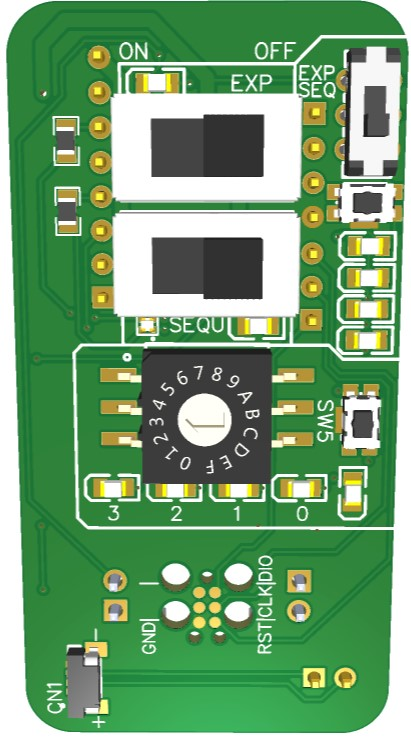
\includegraphics[width=0.45\textwidth]{figures/elec/PCB_IHF.jpg}};
        % \draw[help lines, step=1cm] (-2.5,-4.5) grid (2.5, 4.5);
        % \draw[help lines, step=0.5cm, lightgray] (-2.5,-4.5) grid (2.5, 4.5);
        % \draw[line width=2] (-2.5, +0.0) -- (2.5, +0.0);
        % \draw[line width=2] (+0.0, -4.5) -- (+0.0, +4.5);

        \draw [line width=1, red] (+2.35, +3.90) -| (+1.10, +0.50) -- (+1.75, 0.15) -| (+2.35, +3.9);
        \draw [line width=1, red] (+1.10, +3.60) -| (-1.10, +1.95) -| (+1.10, +3.6);
        \draw [line width=1, red] (+1.10, +1.95) -| (-1.10, +0.65) -| (-0.45, +0.35) -| (+1.10, +1.95);
        \draw [line width=1, red] (+2.25, +0.05) -- (+1.50, +0.05) -- (+0.75, +0.30) -| (-1.50, -1.75) -| (+2.25, +0.05);
        \draw [line width=1, red] (+1.00, -2.00) -| (-0.90, -3.50) -| (+1.00, -2.00);

        \node (bat_lbl)   at (+4.50, +2.50) {Jauge batterie};
        \node (sel_lbl)   at (+4.50, -0.75) {Sélecteur de};
        \node (prog_lbl)  at (+4.50, -1.25) {programme};
        \node (iface_lbl) at (+4.50, -2.75) {Interface de};
        \node (debug_lbl) at (+4.50, -3.25) {débogage SWD};

        \draw [red, ->, line width=0.5] (bat_lbl.west) -- (+2.40, +2.25);
        \draw [red, ->, line width=0.5] (sel_lbl.west) -- (+2.30, -1.00);
        \draw [red, ->, line width=0.5] (iface_lbl.west) -- (+1.05, -2.75);

        \node (sw_exp_1_lbl) at (-4.50, +2.85) {Interrupteur};
        \node (sw_exp_2_lbl) at (-4.65, +2.35) {expérience};
        \node (sw_seq_1_lbl) at (-4.50, +1.25) {Interrupteur};
        \node (sw_seq_2_lbl) at (-4.60, +0.75) {séquenceur};
        \node (led_rgb_lbl)  at (-4.50, -0.50) {LED RGB};
        \node (conn_1_lbl)   at (-4.50, -2.75) {Connecteur};
        \node (conn_2_lbl)   at (-5.07, -3.25) {I2C};

        \draw [red, ->, line width=0.5] (sw_exp_1_lbl.east) -- (-1.15, +2.75);
        \draw [red, ->, line width=0.5] (sw_seq_1_lbl.east) -- (-1.15, +1.25);
        \draw [red, ->, line width=0.5] (led_rgb_lbl.east)  -- (-1.75, +0.50) -- (-0.85, +0.50);
        \draw [red, ->, line width=0.5] (conn_1_lbl.east)   -- (-1.75, -3.50);
    \end{tikzpicture}
    
    \captionof{figure}{PCB \acrlong{IHF}}
    \label{fig:pcb_ihf}
\end{minipage}

\begin{itemize}
    \item Une LED RGB permettant de visualiser l'état du logiciel embarqué du séquenceur. Une multitude de couleurs et de
    clignotement peuvent alors indiquer à quel endroit dans le programme le séquenceur se trouve ; \\
    \item Un sélecteur de programme. Le sélecteur possède 16 positions. Un bouton poussoir permet de déclencher la lecture de la
    position du sélecteur et d'envoyer cette information au séquenceur et ainsi d'effectuer l'action correspondante. 4 leds
    permettent de visualiser la position du sélecteur ; \\
    \item Une interface de débogage \acrshort{SWD} permettant de programmer le microcontrôleur du séquenceur et de déboguer le
    logiciel embarqué alors que la fusée est assemblée. Elle est fait de sorte à ce qu'un câble Tag Connect TC2030 puisse s'y
    connecter ; \\
    \item Un connecteur I2C permettant de connecter le séquenceur à un éventuel système externe. L'idée était de pouvoir
    connecter un module doté d'interface tactile plus simple à utiliser ainsi que d'un écran pour visualiser les informations de
    la fusée et permettre de rendre les opérations au sol encore plus simples et plus intuitives. Le module n'a pas pu être
    développé à temps pour le vol de la fusée SP-02. 
\end{itemize}

\newpage

\begin{figure}[h!]
    \centering
    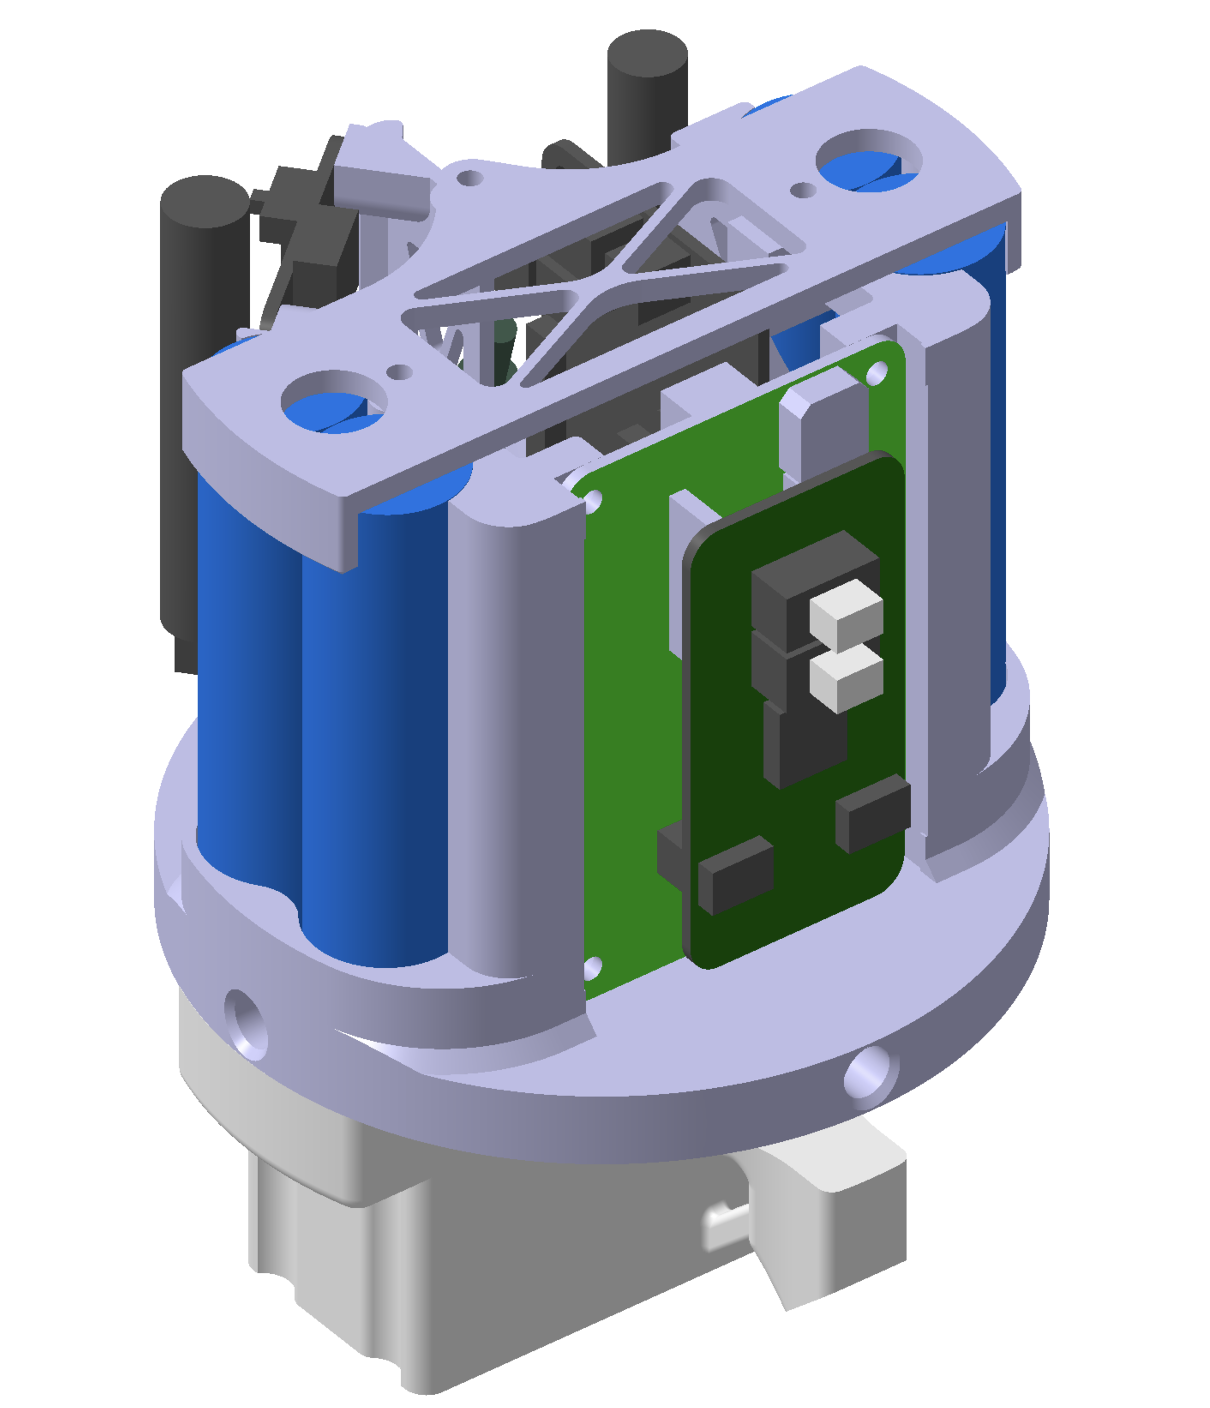
\includegraphics[width=0.5\textwidth]{figures/meca/visu_bloc_elec_1-1.png}
    \caption{Visualisation du séquenceur et de son IHF dans le bol électronique}
    \label{fig:sp02_visu_elec}
\end{figure}

\vfill
